\documentclass[11pt]{article}

\usepackage[margin=1in]{geometry}
\usepackage{amsmath,amssymb}
\usepackage{booktabs}
\usepackage{graphicx}
\usepackage{microtype}
\usepackage[numbers,sort&compress]{natbib}
\usepackage{xcolor}
\usepackage[colorlinks=true,linkcolor=blue!60!black,citecolor=blue!60!black,urlcolor=blue!60!black]{hyperref}
% let \path break at underscores if artifact identifiers are included
\expandafter\def\expandafter\UrlBreaks\expandafter{\UrlBreaks\do\_}

\newcommand{\model}{DABSN}
\newcommand{\vv}[1]{\mathbf{#1}}

\title{One Layer, Both Gaps: A Persistent-Modulation Recurrence that\\
Generalizes Copy \emph{and} Tracks Non-Solvable Group State}
\author{Nicholas Rosdahl\\
Independent Researcher\\
\texttt{nicholasrosdahl@yahoo.com}}
\date{}

\begin{document}
\maketitle

\begin{abstract}
Two failure modes are routinely used to separate sequence-architecture
families. On the \textbf{copy} task, attention re-reads its input losslessly
while any fixed-width recurrence is bandwidth-bound \citep{jelassi2024repeat}.
On non-solvable group word problems such as \textbf{A5} --- NC$^1$-complete state tracking
\citep{barrington1989bounded} --- a genuine sequential nonlinear state is
essential: constant-depth transformers learn only length-bounded shortcuts
\citep{liu2023transformers}, and diagonal selective state-space models are
provably confined to TC$^0$ \citep{merrill2024illusion}. The two gaps pull in
opposite directions and are commonly taken to imply that no single recurrent
layer can hold both. We give a counterexample at the level of one block
design. \model{}, the converged design of the Adaptive Bias State Network
family, stores memory as persistent modulation of a per-unit operating
baseline and exposes, over a single shared content score, three retrieval
primitives plus a nonlinear consolidation recurrence --- each behind a learned
scalar gain initialized so the apparatus begins as a no-op. Trained separately
per task with no structural change, instances
(a)~generalize copy to $50\times$ training length ($0.961 \pm 0.035$ accuracy
at length 3200 over three seeds, where a RoPE transformer collapses to
$0.049$ at $2\times$), and (b)~track the standard A5/60 word problem from
length 256 to length 16{,}384 ($64\times$) with perfect accuracy over two
seeds, while an LSTM trained on the same protocol decays to $0.139$ and RoPE
attention is at chance by length 2048. Removing only the recurrence's
nonlinear state feedback --- the input-controlled TC$^0$ regime, same block and
parameter budget --- collapses A5 to chance even at the training length,
causally isolating the nonlinear state as the mechanism. Reading the converged diagnostics shows the optimizer
selects the appropriate primitive within each training run, the off-task
pathway idling. The same train-short/evaluate-long flatness recurs across
multi-query associative recall, key--value retrieval, burst-anomaly detection,
and character-level language modeling. We argue persistent-modulation memory
is a third substrate, not a recurrence--attention compromise; seed counts and
scope are stated per claim.
\end{abstract}

\section{Introduction}

The dominant sequence architectures are separated by two complementary,
theoretically grounded gaps.

The \textbf{copy} task --- emit the next token of a previously seen stream ---
is the canonical case where attention beats recurrence: a transformer attends
back to the matching position and re-reads it losslessly, so its accuracy is
independent of stream length, whereas a recurrence of width $H$ must compress
the entire history into $H$ numbers and degrades once the content exceeds that
budget \citep{jelassi2024repeat}. Copy is the \emph{memory-bandwidth} corner.

The \textbf{A5 word problem} --- maintain the running product in a
non-solvable permutation group --- is the canonical case where recurrence
beats attention: it is NC$^1$-complete \citep{barrington1989bounded}, so a
constant-depth, log-precision transformer (in TC$^0$) cannot express it at
arbitrary length and instead learns shortcuts that hold only up to the
training length \citep{liu2023transformers}. Crucially, \emph{diagonal/
selective} state-space models such as Mamba \citep{gu2023mamba} are also
confined to TC$^0$ and provably cannot track non-solvable state at growing
length \citep{merrill2024illusion}. This is the \emph{state-tracking} corner.

These two gaps pull in opposite directions --- copy rewards lossless
re-reading, group word problems reward a genuine sequential nonlinear state --- and are
commonly used to argue that the field faces an inherent trade-off: a layer
good at one is structurally bad at the other.

\paragraph{Contribution.} We present a single recurrent block --- one
architecture, trained separately per task with no per-task structural change
--- that closes \emph{both} gaps:

\begin{enumerate}
\item \textbf{Architecture (\S\ref{sec:method}).} \model{} stores memory as
persistent modulation of a per-unit bias baseline, separating the expressed
activation $y_t$ from a persistent bias state $b_t$. Its readout computes one
shared content score and exposes three associative primitives ---
\emph{content}, \emph{induction} (gather the successor of the matched write),
and \emph{position-from-association} --- plus a re-attached nonlinear diagonal
recurrence. Each pathway has a learned scalar gain initialized so the
apparatus begins as a no-op.

\item \textbf{Both gaps, one block design
(\S\ref{sec:copy}--\S\ref{sec:mechanism}).} Trained on copy, the block
generalizes to $50\times$ training length (three seeds) via the induction read
with the recurrence idle; trained on the standard A5/60 word problem, the
\emph{same block design} tracks to $64\times$ training length. These are separately
trained instances of one identical design, not one checkpoint doing both at
once. We read the mechanism directly off the learned gains --- in each
separately trained model the off-task pathway's gain goes to $\approx 0$ ---
and verify it causally by eval-time knockout: zeroing the induction gain
sends a copy-trained checkpoint to exact chance at every length, while
zeroing its other pathways changes nothing.

\item \textbf{Length generalization as an emergent property
(\S\ref{sec:emergent}).} The same train-short/evaluate-long flatness appears
across MQAR, key--value recall, burst-anomaly detection, and character-level
language modeling, where a RoPE transformer cliffs and gated recurrences sit
near chance --- supporting the claim that length-robustness is a property of
the substrate, not a per-task trick.
\end{enumerate}

We are explicit about scope (\S\ref{sec:limitations}): comparisons follow an
each-model-at-its-own-best-config protocol, several rows are single-seed, and
the A5/Mamba separation is theorem-backed rather than measured head-to-head
here.

\section{Related Work}

\paragraph{State-space models and state-tracking.} Structured SSMs (S4, S5)
and selective SSMs \citep{gu2023mamba} achieve strong long-range modeling with
linear-time recurrence, but their diagonal, input-controlled linear state
places them in TC$^0$: \citet{merrill2024illusion} show this excludes
non-solvable group word problems such as A5 at growing length.
\citet{grazzi2024unlocking} extend the reachable class of linear RNNs by
allowing negative eigenvalues, unlocking some state-tracking (e.g., parity),
but non-solvable word problems remain outside fixed-depth diagonal linear
designs. Our A5 result is the complementary positive: a \emph{nonlinear}
recurrence that tracks the standard A5/60 protocol at $64\times$ training length.

\paragraph{Transformers and copy shortcuts.} \citet{jelassi2024repeat} isolate
copy as the regime where attention's lossless re-reading beats recurrence.
\citet{liu2023transformers} show attention learns automaton shortcuts that
fail beyond the training length --- precisely the cliff our RoPE baseline
exhibits at $2\times$ on copy. Our copy result is a recurrence that does
\emph{not} cliff, via an explicit induction read.

\paragraph{Attention--recurrence hybrids.} Griffin/Hawk interleave gated
linear recurrences with local attention \citep{de2024griffin}; Jamba
interleaves Mamba and attention layers \citep{lieber2024jamba}. Such hybrids
can cover both corners \emph{by composition}: two distinct modules, each
paying its own cost, with the division of labor fixed by the architecture.
Extended recurrences --- xLSTM's exponential gating and matrix memory
\citep{beck2024xlstm}, delta-rule fast-weight states
\citep{schlag2021linear,yang2024gated}, RWKV \citep{peng2023rwkv} --- enrich
the recurrent state itself but do not expose an induction-style successor
read. \model{} is neither: a single block, containing no attention layer,
whose retrieval primitives read the recurrence's \emph{own committed writes}
over position-free content keys, with every pathway gated to a no-op at
initialization and adopted only if it reduces task loss
(\S\ref{sec:residual}).

\paragraph{Associative recall and induction.} Multi-query associative recall
\citep{arora2023zoology} is the standard synthetic for in-context retrieval;
induction heads \citep{olsson2022context} are the attention circuit for
``find the previous occurrence and output what followed.'' \model{} bakes an
induction primitive directly into a recurrent block --- the same
match-then-successor computation, but over position-free content keys carried
in recurrent state, which is why it is length-flat.

\paragraph{Fast-weight and modulation memories.} The persistent bias state is
related to fast-weight programmers and gain-modulation memories
\citep{schmidhuber1992learning,ba2016using,schlag2021linear}, but differs in
treating memory as a retention/write/plasticity/budget design space over a
baseline-modulating state, and in exposing multiple read primitives
selectable by the optimizer.

\section{Method}
\label{sec:method}

\subsection{The \model{} state equation}

\model{} separates the \emph{expressed activation} $y_t$ from a
\emph{persistent bias state} $b_t$. The activation expresses the current input
under the present operating conditions; the bias state persists and changes
the conditions under which future activations form. The family is one
template:
\begin{align}
y_t &= \tanh(W x_t + b_t) \nonumber\\
b_{t+1} &= R_t \odot b_t + \beta + M_t \odot (A\,y_t), \qquad b_0 = 0,\; y_0 = 0
\end{align}
with a \emph{retention} operator $R_t$, a \emph{write/plasticity} operator
$M_t$, a learned baseline $\beta$, and activity-to-bias feedback $A\,y_t$.
The separation is not notational: in the family's lineage, decoding the
output from $b_T$ alone outperforms decoding from $y_T$ alone on memory
tasks (with the concatenation $[y_T, b_T]$ best when stored memory must be
interpreted through current context) --- direct evidence that the persistent
state, not the expressed activation, is what carries the memory. Variants of
the family differ in $R_t$ and $M_t$; the converged design used throughout
this paper is the budgeted, admission-gated member described next.

\subsection{The governor core: budgeted, gated plasticity}
\label{sec:governor}

At each step, an admission gate $s_t$, a novelty trace $n_t$, a slow
saturation trace $c_t$, and an energy budget $e_t \in [0,1]$ co-regulate
plasticity:
\begin{align}
s_t &= \mathrm{hardsigmoid}(W_g x_t + U_g y_t) && \text{write admission} \nonumber\\
n_t &= \tanh(|A\,y_t - b_t|) && \text{novelty} \nonumber\\
c_t &= \rho_c\, c_{t-1} + (1-\rho_c)\,[\,n_t (1 - e_t)\,] && \text{saturation (slow)} \nonumber\\
n_t^{\mathrm{eff}} &= n_t \,(1 - \sigma(\theta_s)\, c_t) && \text{saturation downregulates novelty} \nonumber\\
p_t &= s_t \, e_t && \text{plasticity} = \text{admission} \times \text{budget} \nonumber\\
b_{t+1} &= (1-\alpha)\, b_t + \beta + \lambda\,(p_t \cdot A\,y_t) && \text{write into persistent memory} \nonumber\\
e_{t+1} &= \mathrm{clamp}\big(e_t + r_t (1 - e_t) - k_t\, p_t,\; 0,\; 1\big) && \text{spend-and-recover budget} \nonumber\\
m_t &= p_t \cdot (A\,y_t) && \text{the committed write}
\end{align}
$m_t$ is the object every downstream memory reads. The write cost $k_t$ and
recovery $r_t$ are exp-tanh functions of $(s_t, y_t, b_t, n_t^{\mathrm{eff}},
c_t)$.

\subsection{The unified read: one score, three primitives}
\label{sec:read}

Over an admitted set of writes (admission below), a single content score is
computed once and shared by three reads that differ only by an added term and
by which value bank they gather (all causal-masked, softmax over admitted
$j$):
\begin{align}
q_i &= \mathrm{normalize}(A\,y_i), \quad k_j = \mathrm{normalize}(m_j), \quad
\mathrm{scale} = (\mathrm{softplus}(\log\text{-temp}) + 1)\sqrt{H} \nonumber\\
\mathrm{content}[i,j] &= \mathrm{scale}\cdot (q_i \cdot k_j) + \mathrm{keybias}_j \nonumber\\
\mathrm{sig}[i,j] &= g_{\mathrm{sig}}\, (\xi_i \cdot \xi_j), \qquad
\xi_t = \mathrm{normalize}([\bar e_t, \bar c_t, \bar n_t, \bar p_t]) \in \mathbb{R}^4 \nonumber\\[2pt]
\mathrm{SHORT}_i &: \mathrm{softmax}_j(\mathrm{content} + \mathrm{adm}_j),
  \;\text{values } m_j, \;\text{mask } j \le i \nonumber\\
\mathrm{PERM}_i &: \mathrm{softmax}_j(\mathrm{content} + \mathrm{sig} + \mathrm{adm}_j),
  \;\text{values } m_j, \;\text{mask } j \le i \nonumber\\
\mathrm{INDUCT}_i &: \mathrm{softmax}_j(\mathrm{content} + \mathrm{adm}_j),
  \;\text{values } m_{j+1}, \;\text{mask } j < i \nonumber\\[2pt]
\mathrm{retrieved}_i &= g_{\mathrm{short}}\,\mathrm{SHORT}_i + g_{\mathrm{perm}}\,\mathrm{PERM}_i + g_{\mathrm{ind}}\,\mathrm{INDUCT}_i
\end{align}

\begin{itemize}
\item \textbf{Content/PERM} read the matched write (the token itself) using a
position-free content key plus a \emph{position-from-association} key $\xi$
--- the \emph{trace signature}, read off the recurrence's own internal traces.
The state is the position; there is no positional encoding.
\item \textbf{Induction} keeps the same content match but gathers the
\emph{successor} $m_{j+1}$ under a strict-causal mask ($j < i$, so $j{+}1 \le
i$ is available): ``find where this token occurred before, output what
followed it.'' This is the copy primitive; the plain content read returns the
matched token itself, which is useless when the task is to emit the
\emph{next} token.
\end{itemize}

\paragraph{Admission.} Each write carries a score $\mathrm{adm}_j$ computed
from the full set of internal traces (plasticity, novelty, saturation,
budget); only writes within a \emph{learned relative window} of the
per-sequence best are readable:
$\mathrm{member}_j = [\,\mathrm{adm}_j \ge \max_k \mathrm{adm}_k -
\mathrm{softplus}(w)\,]$, with $w$ initialized wide. The window is relative,
so the admitted set never collapses to one write and never starves the read;
the admitted size $n_{\max}$ emerges per task ($\approx T$ on incompressible
copy, small on selective recall), making the read $O(T \cdot n_{\max})$
rather than $O(T^2)$.

\paragraph{Memory scaling.} The admitted write set is the block's readable
memory, and its size is task-adaptive by design. On incompressible copy this
is information-theoretically forced: emitting $T$ tokens losslessly requires
$T \log_2 |V|$ recoverable bits, which no fixed-width state can hold, so the
admitted set grows to $\approx T$ and the fixed-width bandwidth bound of
\citet{jelassi2024repeat} is sidestepped rather than contradicted --- that
bound applies to recurrences that compress history into $H$ numbers, and on
copy \model{} does not. On selective-recall tasks the admitted set stays
small and the block operates as a compact recurrence. What is constant across
both regimes --- and what we argue produces the length-flatness --- is the
\emph{addressing}: retrieval into the admitted set is purely
content-and-trace-based, with no positional table of any kind, so nothing in
the read mechanism is calibrated to the training length. The copy claim of
this paper should be read accordingly: not that a fixed-width state beats the
bandwidth bound, but that position-free addressing over state-carried writes
removes the length cliff that positional addressing exhibits.

\subsection{The recurrence: an explicit nonlinear scan}
\label{sec:recurrence}

The unified read is purely associative and has no sequential nonlinear state,
so it cannot track non-solvable group composition at length. A gated
consolidation recurrence is therefore attached as an explicit diagonal scan
in hidden space:
\begin{align}
\mathrm{expected}_t &= \rho_e\, \mathrm{expected}_{t-1} + (1-\rho_e)\, m_t \nonumber\\
\mathrm{pe}_t &= \tanh(|m_t - \mathrm{expected}_{t-1}|) && \text{surprise} \nonumber\\
a_t &= \rho_a\, a_{t-1} + (1-\rho_a)(1 - \mathrm{pe}_t), \quad a_0 = 1 && \text{confidence trace} \nonumber\\
\mathrm{eff}_t &= \mathrm{retain} + (1 - \mathrm{retain})\cdot g_a \cdot a_t && \text{retention gate} \nonumber\\
\mathrm{long}_t &= \mathrm{eff}_t\, \mathrm{long}_{t-1} + (1 - \mathrm{eff}_t)\,(p_t \cdot \mathrm{pe}_t \cdot m_t) \nonumber\\
\mathrm{read}_t &= \mathrm{out}_t + g_{\mathrm{rec}}\, \mathrm{long}_t
\end{align}
Because this is a diagonal linear-state primitive, a fused GPU scan kernel
reproduces it exactly (verified against a CPU gradient check).

\subsection{The gated residual and superset-at-init}
\label{sec:residual}

All retrieval is folded into the core through one gated residual
$z_t = y_t + \gamma\,\mathrm{read}_t$, with $\gamma$ initialized near zero.
At initialization the entire read/recurrence apparatus is a
no-op ($z_t \approx y_t$); training dials it in per task. Every added pathway
(induction, recurrence, trace signature) likewise begins inert via its gain,
so a pathway is adopted only if it reduces loss. This makes the design
lineage itself an ablation grid: each component was added inert against the
previous family member and benchmarked across the task matrix, so a stage
that did not help would simply have trained back to its inert initialization
--- that each was instead adopted, and improved on its predecessor, is
per-component evidence of contribution. \textbf{No mechanism routes the
reads by task} --- the gains are ordinary learned parameters.

\section{Experimental Setup}
\label{sec:setup}

\paragraph{Model.} \model{} in its \emph{sequence} (seq) read geometry ---
the geometry this paper describes. Compact copy/recall stress configs use
approximately 17--31k parameters depending on hidden width ($h48$--$h96$)
and task head; the standard A5/60 headline uses the wider $h256$,
\texttt{seq:256:256} config with 378{,}198 parameters. The \emph{field} and
\emph{hybrid} variants appearing in the three-seed stress pass
(\S\ref{sec:emergent}) change only the read geometry over the same block. The
verified-CSV model names \texttt{dabsn\_seq}, \texttt{dabsn\_field}, and
\texttt{dabsn\_hybrid} denote this same architecture; internal implementation
names in archival logs are mapped to this public model name.

\paragraph{Protocol.} Each model is run at its own best configuration --- the
fair protocol for a family whose empirical sweet spot is low hidden width
with a higher learning rate; gated-recurrent and attention baselines prefer
lower learning rates. Train at a short length, evaluate at multiples of it
(train-short/evaluate-long). Chance is reported per task, and seed counts are
stated per result.

\paragraph{Baselines.} GRU, LSTM, and transformers with absolute and RoPE
(relative) positional encodings. We treat RoPE as the primary attention
opponent deliberately: the absolute-PE transformer falls to chance the
instant evaluation exceeds training length, whereas RoPE extrapolates far
better and is the honest opponent.

\section{Results}

\subsection{Copy --- the memory-bandwidth gap (induction read)}
\label{sec:copy}

Copy is fed $x_k$ and must emit $x_{k+1}$. The plain content read literally
cannot answer it (it returns the matched token); with the induction read,
copy is length-flat. Table~\ref{tab:copy} reports the three-seed verified
pass at vocabulary 64, $h48$, train length 64, evaluated to $50\times$;
Figure~\ref{fig:bothgaps} (left) plots the full curves.

\begin{table}[t]
\centering
\caption{Copy accuracy vs.\ evaluation length (vocab 64, train length 64,
$h48$, 1000 steps; mean $\pm$ std over 3 seeds). Chance $= 1/64 = 0.0156$.
GRU and LSTM sit at chance at every length above the training length
(Fig.~\ref{fig:bothgaps}). Machine-readable result tables are included as
ancillary CSV files with this release.}
\label{tab:copy}
\small
\begin{tabular}{lccccccc}
\toprule
eval length & 64 & 128 ($2\times$) & 256 & 512 ($8\times$) & 1024 & 2048 & 3200 ($50\times$) \\
\midrule
\textbf{\model{} (seq)} & $.985$ & $.992$ & $.996$ & $.997$ & $.995$ & $.984$ & $\mathbf{.961 \pm .035}$ \\
Transformer (RoPE) & $1.000$ & $.049 \pm .014$ & $.063$ & $.046$ & $.033$ & $.025$ & $.022 \pm .001$ \\
\bottomrule
\end{tabular}
\end{table}

The RoPE transformer solves the training length perfectly and collapses at
$2\times$; \model{} holds $0.96$--$1.00$ out to $50\times$. A converged
single-seed run at $h96$ (4000 steps) reaches accuracy $0.9999$, $0.9999$,
$0.9994$, and $0.9990$ at lengths 64, 128, 256, and 512. The
field-geometry variant of the same block reaches
$0.992 \pm 0.004$ at $50\times$, so the behavior is a property of the block,
not of one read geometry.

\begin{figure}[t]
\centering
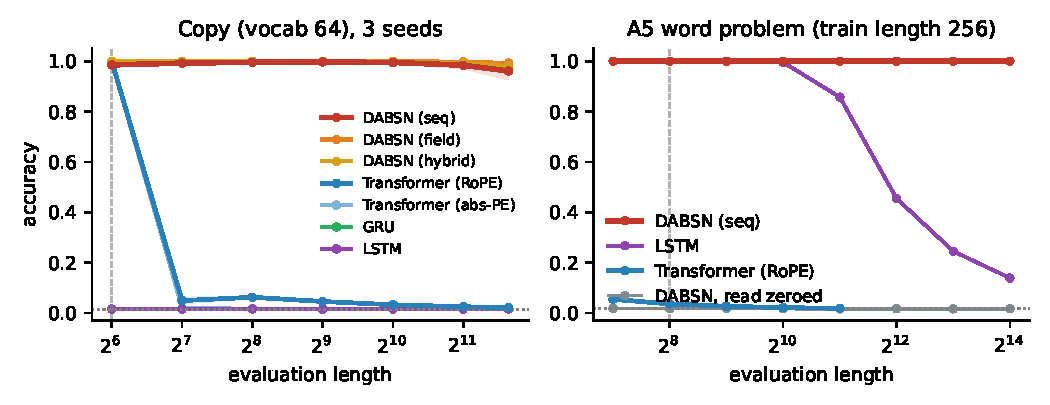
\includegraphics[width=\linewidth]{figs/fig1_both_gaps.pdf}
\caption{\textbf{One block design, both gaps.} Left: copy accuracy vs.\
evaluation length (train length 64, vocab 64; mean $\pm$ std, 3 seeds).
Attention (RoPE) collapses at $2\times$; gated recurrences (GRU/LSTM) sit at
chance; \model{} is length-flat to $50\times$. Right: standard A5/60
word-problem accuracy (dense 60-way supervision; train length 256, single
seed). \model{} remains perfect to length 16{,}384 ($64\times$), while the
LSTM positive control decays at long length and RoPE attention is at chance.
``\model{}, read zeroed'' is an eval-time causal control: the same trained
checkpoint re-evaluated with the gated-residual read gain $\gamma$
(\S\ref{sec:residual}) zeroed, removing the entire retrieval output at once
(all primitives and the consolidation channel; distinct from the per-pathway
gain knockouts of Table~\ref{tab:knockout}). Accuracy falls to chance at
every length: the tracked state is expressed through the read pathway, and
the intact curve is not an artifact of the task head.}
\label{fig:bothgaps}
\end{figure}

\subsection{A5 --- the standard state-tracking gap (recurrence)}
\label{sec:s5}

A5 supervises the running group product densely (60-way classification at
every position, no final-state shortcut). The A5 run uses the same block
design, trained separately with train length 256, cosine-decayed learning
rate $0.003$, 60{,}000 steps, $h256$ and DABSN layer spec
\texttt{seq:256:256}; chance $= 1/60 = 0.0167$:

\begin{table}[h]
\centering
\caption{A5/60 accuracy vs.\ evaluation length, from the machine-readable
ancillary result tables. \model{} (seq) is two-seed (both seeds identical to
the reported precision); the linear-state ablation is the seed-1
input-controlled (TC$^0$) variant of the same block. LSTM/RoPE are the
single-seed headline baselines.}
\label{tab:s5}
\small
\begin{tabular}{lcccccccc}
\toprule
eval length & 128 & 256 & 512 & 1024 & 2048 & 4096 & 8192 & 16384 ($64\times$) \\
\midrule
\textbf{\model{} (seq)} & $1.000$ & $1.000$ & $1.000$ & $1.000$ & $1.000$ & $1.000$ & $1.000$ & $\mathbf{1.000}$ \\
\model{}, linear-state & $0.036$ & $0.026$ & $0.022$ & $0.019$ & $0.018$ & $0.017$ & $0.017$ & $0.017$ \\
LSTM & $1.000$ & $1.000$ & $1.000$ & $0.995$ & $0.857$ & $0.455$ & $0.245$ & $0.139$ \\
Transformer (RoPE) & $0.054$ & $0.036$ & $0.027$ & $0.021$ & $0.019$ & skipped & skipped & skipped \\
\bottomrule
\end{tabular}
\end{table}

\model{} is length-flat through length 16{,}384, while the LSTM positive
control learns the training distribution perfectly but decays after the
training horizon. RoPE attention is already near chance by length 2048 and
longer attention evals are skipped by the configured T4 quadratic-attention
budget.

\paragraph{Second seed.} A second training run at seed~1, identical
\texttt{seq:256:256} config, reproduces the headline exactly: $1.000$ at every
length from $128$ to $16{,}384$ ($64\times$), matching seed~0
(Fig.~\ref{fig:s5ablation}, left). The A5/60 result is thus two-seed, not
single-seed.

\paragraph{The nonlinear state is necessary: a linear-state ablation.} The
theory attributes A5 to the block's \emph{nonlinear} sequential state
(\S\ref{sec:recurrence}); we test this causally by removing that nonlinearity
and nothing else. In the linear-state variant every transition coefficient of
the core scan is a function of the input alone --- the persistent state $b_t$
never feeds back into the gates, novelty, energy law, or write --- so the state
evolves as a diagonal linear system with input-controlled coefficients, the
regime \citet{merrill2024illusion} place in TC$^0$. The parameter count,
learning rate, step budget, and length curriculum are unchanged
(\texttt{seq:256:256}, $378{,}198$ params, seed~1). The ablated block does not
merely lose length generalization --- it never learns A5 \emph{at all},
sitting at chance at the training length ($0.026$ train accuracy) and at every
evaluation length (Fig.~\ref{fig:s5ablation}, right; Table~\ref{tab:s5}). With
every other factor held fixed, deleting the nonlinear state feedback destroys
the capability outright, demonstrating --- rather than inferring by
elimination (\S\ref{sec:mechanism}) --- that the nonlinear recurrence, not the
reads or the parameter budget, is what tracks A5.

\begin{figure}[t]
\centering
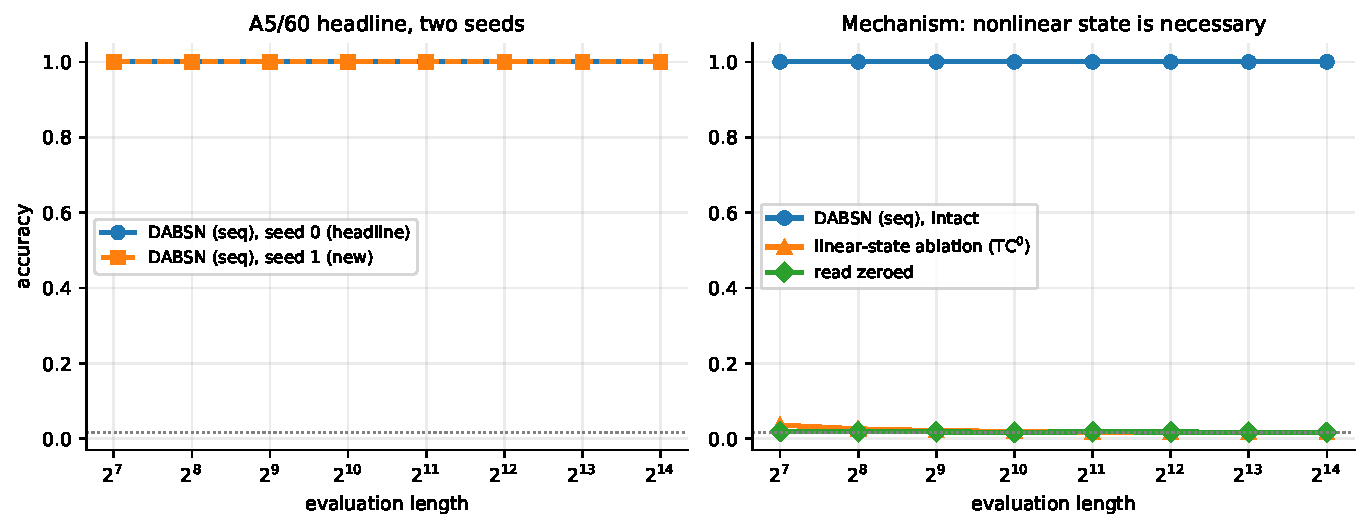
\includegraphics[width=\linewidth]{figs/fig3_a5_seed_ablation.pdf}
\caption{\textbf{A5/60: two-seed reproduction and the linear-state ablation.}
Left: the \texttt{seq:256:256} block is perfect and length-flat to $64\times$
at both seeds (seed~0 headline, seed~1 new run). Right: two causal controls on
the seed-1 checkpoint. The input-controlled \emph{linear-state} ablation of the
same block (the TC$^0$ regime of \citet{merrill2024illusion}) fails to learn
A5 even at the training length, and the ``read zeroed'' control
(\S\ref{sec:residual}) is at chance; the intact block is at $1.000$ throughout.
Chance $=1/60=0.0167$.}
\label{fig:s5ablation}
\end{figure}

\subsection{Mechanism: the optimizer picks the primitive}
\label{sec:mechanism}

Nothing routes the reads --- the gains are ordinary learned parameters --- yet
each separately trained model recruits only the pathway its task needs. We show
this two ways: causally on the A5/60 headline itself, and as a per-pathway
double dissociation on copy.

\paragraph{A5/60: the nonlinear state carries it.} The two ablations of
\S\ref{sec:s5} establish the state-tracking mechanism directly on the A5/60
checkpoint. Removing the nonlinear state feedback (the linear-state variant)
collapses A5 to chance even at the training length, and zeroing the whole read
pathway (read zeroed) is likewise at chance. The capability needs both the
block's nonlinear recurrent state and the read that expresses it; no
associative read alone suffices, exactly as the theory requires
(\S\ref{sec:recurrence}), because the unified read has no sequential nonlinear
state and cannot carry non-solvable composition at growing length.

\paragraph{Copy: a per-pathway double dissociation.} On copy the assignment is
visible in the converged gains and confirmed causally by knockouts. The
induction gain trains up ($0.1 \to 0.79$) while the recurrent consolidation
channel stays idle ($g_{\mathrm{rec}} = 0.017$) --- expected, since the content
read returns the matched token rather than its successor, so only the induction
read can emit the \emph{next} token (\S\ref{sec:read}). Eval-time knockouts
zero one pathway gain on the trained checkpoint, all other weights untouched
(Table~\ref{tab:knockout}).

\begin{table}[h]
\centering
\caption{Eval-time knockout of one pathway gain on the same trained copy
checkpoint (verified-stress config: $h48$, train length 64, 1000 steps, single
seed, evaluated to length 512; chance $= 0.0156$). Zeroing the induction gain
sends copy to chance; zeroing the consolidation or signature gain changes
nothing. Machine-readable result tables are included as ancillary CSV files
with this release.}
\label{tab:knockout}
\small
\begin{tabular}{llcccc}
\toprule
task & condition & 64 & 128 & 256 & 512 \\
\midrule
copy & intact & $0.985$ & $0.992$ & $0.996$ & $0.997$ \\
 & $g_{\mathrm{ind}} = 0$ & $\mathbf{0.017}$ & $\mathbf{0.016}$ & $\mathbf{0.015}$ & $\mathbf{0.016}$ \\
 & $g_{\mathrm{rec}} = 0$ & $0.985$ & $0.992$ & $0.996$ & $0.997$ \\
 & $g_{\mathrm{sig}} = 0$ & $0.985$ & $0.992$ & $0.996$ & $0.997$ \\
\bottomrule
\end{tabular}
\end{table}

Zeroing the induction gain sends copy to exact chance at every length, while
zeroing the consolidation channel or the trace signature changes nothing --- a
full double dissociation: the induction read is necessary, and the recurrent
consolidation channel is causally inert on copy, exactly as the gain values
indicated. The two results together are the mechanism claim in its sharpest
form: copy is solved by a single discrete, removable primitive --- the
induction read --- while state tracking is solved by the nonlinear state
itself, a substrate no read gain can remove because it is not a pathway.
Deleting the state's nonlinear feedback destroys A5 outright (\S\ref{sec:s5});
deleting the induction read destroys copy; and in each model the off-task
pathway is idle. One block; the optimizer recruits the right computation per
task, with no mechanism routing the reads.

\subsection{Length generalization is an emergent property}
\label{sec:emergent}

The same train-short/evaluate-long flatness appears across unrelated task
families (each model at its own config; chance noted):

\begin{table}[h]
\centering
\caption{Emergent length-flatness across task families (single-seed
converged runs; see Table~\ref{tab:verified} for the 3-seed pass). On
character LM, \model{} trails RoPE \emph{in-distribution} at context 128 by
$0.057$ bpc --- the win is out-of-distribution length robustness, not
in-distribution quality.}
\label{tab:families}
\small
\begin{tabular}{llclc}
\toprule
Task & train$\to$eval & factor & \model{} & best baseline \\
\midrule
MQAR (recall) & 64$\to$2000 & $31\times$ & $1.000$ & RoPE $0.178$; abs-PE chance \\
Key--value ($h16$) & 64$\to$512 & $8\times$ & $1.000$ & GRU $0.081$; transf.\ $0.055$ \\
Burst-anomaly ($h16$) & 64$\to$1024 & $16\times$ & $1.000$ & transf./LSTM/coRNN $\approx 0.49$ \\
Char-LM (Shakespeare) & 128$\to$2048 & $16\times$ & bpc $\approx 2.37$ ($\approx$flat) & RoPE $5.86$ (near-random) \\
\bottomrule
\end{tabular}
\end{table}

\begin{figure}[t]
\centering
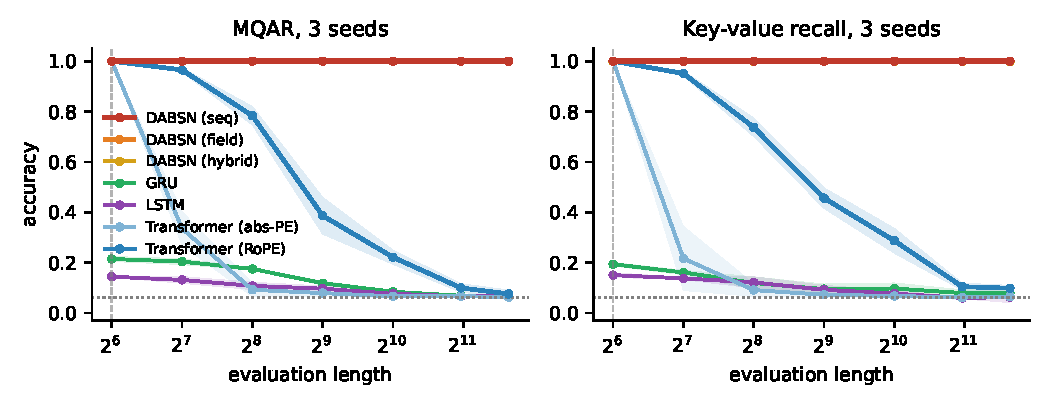
\includegraphics[width=\linewidth]{figs/fig2_recall_50x.pdf}
\caption{\textbf{Verified 3-seed stress pass to $50\times$.} MQAR (left) and
key--value recall (right), train length 64, $h48$, evaluated to length 3200.
All three \model{} read geometries hold $1.000 \pm 0.000$ (one hybrid
key--value seed dips to $0.992$); RoPE decays toward chance; GRU/LSTM/abs-PE
sit at chance.}
\label{fig:recall}
\end{figure}

\paragraph{Verified three-seed stress pass.} After the initial draft, we ran
a three-seed length stress pass on the \model{} read geometries at $h48$,
train length 64 (Table~\ref{tab:verified}, Fig.~\ref{fig:recall}). These are
not the same checkpoints as the converged headline runs above; they verify
that the length-flat behavior of the block is not a single lucky seed and is
shared across its read geometries.

\begin{table}[h]
\centering
\caption{Verified 3-seed length stress at $50\times$ ($h48$, train length 64;
mean $\pm$ std, $n{=}3$). Copy/MQAR use 1000 training steps; key--value uses
2000. The machine-readable result tables record exact steps, seeds, learning
rates, and run identifiers. Chance: $0.0156$ copy, $0.0625$ MQAR/KV.}
\label{tab:verified}
\small
\begin{tabular}{llcc}
\toprule
Task & geometry & \model{} at $50\times$ & best baseline at $50\times$ \\
\midrule
Copy (vocab 64) & seq & $0.961 \pm 0.035$ & RoPE $0.022 \pm 0.001$ \\
 & field & $0.992 \pm 0.004$ & \\
MQAR & seq/field/hybrid & $1.000 \pm 0.000$ & RoPE $0.076 \pm 0.015$ \\
Key--value & seq/field & $1.000 \pm 0.000$ & RoPE $0.098 \pm 0.011$ \\
\bottomrule
\end{tabular}
\end{table}

Each benchmark trains each model from scratch on the short horizon, then
evaluates that same instance zero-shot at longer horizons on the same task
generator and scoring rule: copy supervises only the output-copy positions,
MQAR scores only query positions, and key--value scores the final queried
value. The \model{} rows differ only in read geometry; baselines use the same
input stream and task head. The interpretation is mechanistic: attention
re-derives bindings from positions it was never trained on and decays;
\model{} carries the binding in recurrent state, so length is irrelevant.

\section{Discussion}

The standard framing treats the copy and state-tracking gaps as evidence for a
trade-off: a layer optimized for lossless re-reading is structurally poor at
sequential nonlinear state, and vice versa. Our result is that a single
persistent-modulation recurrence holds both, because it carries two distinct
computational primitives in one block --- an associative induction read and a
nonlinear diagonal recurrence --- and lets the optimizer weight them per
task. The induction read supplies the lossless ``re-read the successor''
operation copy needs without a positional table; the nonlinear recurrence
supplies the genuine sequential state A5 needs without attention's
length-bounded shortcut. Because the off-task pathway goes idle --- and
knockout shows it is causally inert, not merely down-weighted
(\S\ref{sec:mechanism}) --- this is not an ensemble paying for both at once; it
is one substrate expressing the right computation.

A natural objection is that any attention--recurrence hybrid
\citep{de2024griffin,lieber2024jamba} also covers both corners. The
distinction is structural. A hybrid composes two modules --- a softmax
attention layer over token embeddings and a separate recurrent layer --- with
the division of labor fixed by the architecture, and it inherits attention's
positional length-cliff on copy-style re-reading (Table~\ref{tab:copy}).
\model{} contains no attention layer: its reads gather the recurrence's own
committed writes $m_j$ under one shared content score; the keys are
position-free functions of recurrent state, so nothing in the read references
absolute or relative position; the read is admission-bounded rather than
dense; and the entire apparatus is gated to a no-op at initialization, so
each primitive is \emph{recruited by the optimizer}, not allocated by the
designer. The observable consequence is exactly the experiment: the module
hybrids inherit for re-reading cliffs at $2\times$, while the induction read
is flat at $50\times$.

We therefore read the evidence as: \textbf{persistent-modulation memory is a
third substrate}, distinct from ``attention that trades away state'' and
``recurrence that trades away recall,'' rather than a compromise between
them. The emergent length-flatness across four further task families
(\S\ref{sec:emergent}) is consistent with this: length-robustness follows
from carrying bindings in state rather than re-deriving them from position.

\section{Limitations}
\label{sec:limitations}

\begin{enumerate}
\item \textbf{Seeds.} A5/60 state tracking is now two-seed (both seeds perfect
and length-flat to $64\times$; \S\ref{sec:s5}, Fig.~\ref{fig:s5ablation}).
Burst-anomaly and character LM remain single-seed. The $h96$ copy headline is
single-seed, but the verified $h48$ copy, MQAR, and key--value stress passes
are 3-seed. Single-seed rows are \emph{demonstrated, not proven}; wider seed
counts on the remaining single-seed rows are the primary hardening step.
\item \textbf{Protocol.} Comparisons are each-model-at-its-own-best-config.
This is the fair protocol for a low-hidden/high-LR family, but rankings are
configuration-dependent; a single shared grid would not reproduce them. A
matched-config baseline sweep is an immediate next step.
\item \textbf{The Mamba comparison is theorem-backed}
\citep{merrill2024illusion}, not a measured head-to-head here; we cite the
impossibility result rather than running Mamba on A5.
\item \textbf{Mechanism evidence.} On the A5/60 headline the state-tracking
mechanism is shown directly and causally: the linear-state ablation and the
read-zeroed control each collapse it to chance (\S\ref{sec:s5},
Fig.~\ref{fig:s5ablation}). The copy-side per-pathway double dissociation
(Table~\ref{tab:knockout}) is single-seed and evaluated to length 512;
extending it to the $16\times$ horizon, and logging the per-pathway gains on
the A5/60 run itself, are straightforward future hardening.
\item \textbf{Scope.} Copy is shown at vocabulary 64 only. MQAR has a sharp
solve/no-solve basin and CUDA is not fully deterministic under seeding; the
verified pass solves all three seeds to $50\times$, but larger seed counts
remain future hardening.
\item \textbf{Speed.} The implementation includes fused scan/read kernels,
but this paper does not report a controlled throughput or latency study. No
speed comparison with vendor GRU/LSTM is claimed; kernel performance remains
implementation- and hardware-dependent.
\end{enumerate}

\section{Availability}

Machine-readable result tables for this paper are included as ancillary CSV
files. The public code repository is
\url{https://github.com/BleedingXiko/dabsn}. It includes the framework source,
native C++/OpenMP and Triton/CUDA kernels, package tests, runnable paper
reproductions, machine-readable results, and paper build source. Checkpoints
and full training artifacts are retained by the author and are available on
reasonable request.

\bibliographystyle{unsrtnat}
\bibliography{refs}

\end{document}
